\clearpage
\twocolumn[{%
\rqparent
\subsection{SNR as a surrogate for decision accuracy}
\label{app:rq04_surrogates}

\noindent\begin{minipage}[t]{0.485\textwidth}
\vspace{0pt}
\paragraph{Research Question.} \emph{Before the reference is trained, can a statistic computed on the proxy alone tell us whether the proxy's decision will match the reference's? First, which of the 22 SNR definitions of the noise-and-SNR analysis correlates best with \textbf{decision accuracy} across the ladder's languages, and does the answer survive a change of training seed?}

\paragraph{Setup.} For each of 22 SNR definitions, we correlate log$_{10}$ SNR with decision accuracy (Pearson r) across the tasks of one language, on every design pair (multi-axis) and pooling the proxy sizes 90M--1B. We use the seed-1904 runs of every cell, 90M--1.7B. The tasks are those above chance at the proxy and, for DA-size, at 1.7B, plus the bBPB twins and the per-language BPB, which have no chance level. The four discrepancy definitions are undefined off [0, 1], so they read the accuracy tasks alone, a smaller population than the other 18. We also read the accuracy tasks and the bBPB twins apart (Figure~\ref{fig:app_rq04_surrogates_by_scoring}), and the single-axis pairs alone (Figure~\ref{fig:app_rq04_surrogates_mono_axis}). A language needs at least three tasks. Each definition divides a spread of the final scores over the design variants at a size by the checkpoint noise of the last 20 \% of the runs, relative to the mean window score (to the mean depth for \texttt{tukey} and \texttt{projection}). We average the per-language correlation over the languages with at least three tasks (all 50 trained languages, 48--49 for the discrepancy definitions), for DA-size (proxy final against 1.7B final) and DA-ckpt (a proxy's nine early checkpoints, 10--90 \%, against its own final).
\end{minipage}\hfill
\begin{minipage}[t]{0.485\textwidth}
\vspace{0pt}
\begin{rqfinding}
\textbf{1. The relative-spread SNR definitions track decision accuracy best, as a block.} \texttt{rel\_std}, \texttt{rel\_mpd} and \texttt{rel\_dispersion} read mean r 0.51--0.52 with DA-size and 0.55--0.56 with DA-ckpt (0.53--0.54 overall), ahead of \texttt{iqr} (0.51) and the eight dispersion and robust definitions (\texttt{aad}, \texttt{rms\_deviation}, \texttt{dist\_std}, \texttt{mpd}, \texttt{range}, \texttt{dispersion}, \texttt{quartile\_deviation}, \texttt{mad}: 0.48--0.50 overall). (Figure~\ref{fig:app_rq04_surrogates}.)
\\
\\
\textbf{2. No exact definition is best everywhere.} Per language the winner is one of 11 definitions under DA-size and one of 12 under DA-ckpt.
\\
\\
\textbf{3. On the few languages the seed holdout can read (one under DA-size, two under DA-ckpt), it keeps the global ranking, but the per-language picks agree only under DA-size.} The global ranking of the 22 definitions correlates across the seed split at Spearman $\rho$ 0.72 under DA-ckpt and 0.55 under DA-size (on the holdout DA-size is 175M $\rightarrow$ 600M).
\end{rqfinding}
\end{minipage}

\vspace{\baselineskip}
\noindent\begin{minipage}{\textwidth}
\centering
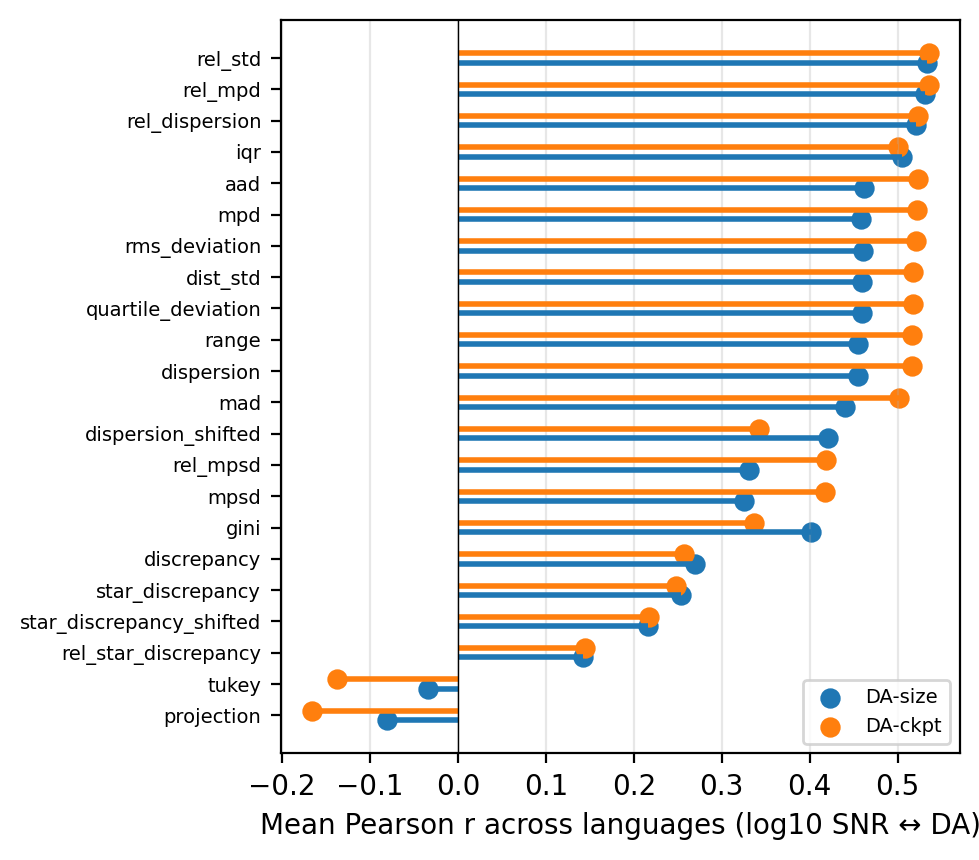
\includegraphics[width=\textwidth,height=0.36\textheight,keepaspectratio]{figures/app_rq04_surrogates.png}
% source: src/signal-and-noise/analysis/rq04_surrogates/pretraining/predictivity/top_variants_overall_paper.png
\captionof{figure}{\textbf{The relative-spread SNR definitions track decision accuracy best, as a block.} For each of the 22 SNR definitions, the mean over languages of the Pearson r between log$_{10}$ SNR and decision accuracy across the tasks of one language, for DA-size (blue) and DA-ckpt (orange). The definitions are ordered by their DA-size correlation.}
\label{fig:app_rq04_surrogates}
\end{minipage}
}]

\begin{figure*}[p]
\centering
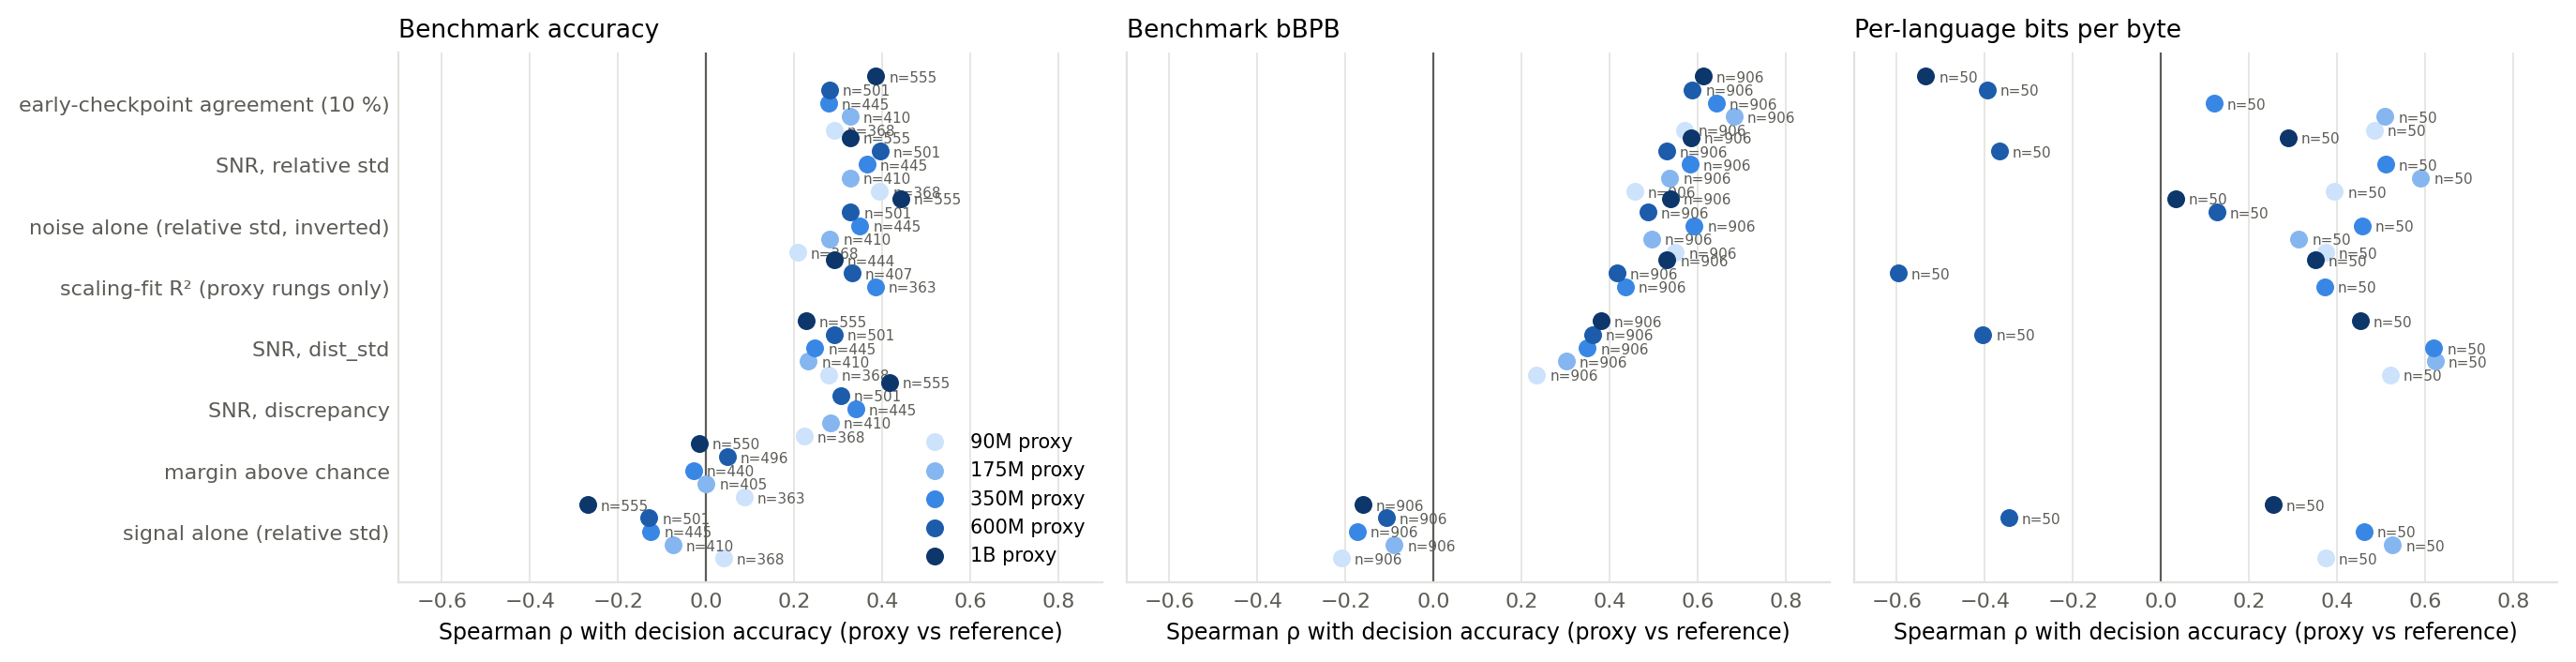
\includegraphics[width=\textwidth,height=0.8\textheight,keepaspectratio]{figures/app_rq04_surrogates_by_scoring.png}
% source: src/signal-and-noise/analysis/rq04_surrogates/pretraining/predictivity/rq3_surrogates_by_scoring_paper.png
\caption{\textbf{The bBPB twins carry most of the pooled association of Figure~\ref{fig:rq3} and the lead of early-checkpoint agreement, while on accuracy alone the relative-standard-deviation SNR leads at 90M, 175M, 600M ($\rho$ 0.33--0.39).} Spearman $\rho$ between each surrogate statistic and DA-size against the 1.7B reference, at each proxy size, for the benchmark tasks above chance scored by accuracy (left), their bBPB twins (middle) and the per-language bits per byte of the 50 trained languages (right). The number next to each point is the number of tasks. On the twins early-checkpoint agreement reads 0.57--0.68 and the SNR 0.46--0.58, against 0.28--0.39 and 0.33--0.39 on accuracy. On the per-language bits per byte 5 of the 6 statistics turn negative at 600M. SNR discrepancy and the margin above chance are defined on the accuracy tasks only, and the scaling-fit $R^2$ needs three model sizes, so it starts at 350M.}
\label{fig:app_rq04_surrogates_by_scoring}
\end{figure*}

\begin{figure*}[p]
\centering
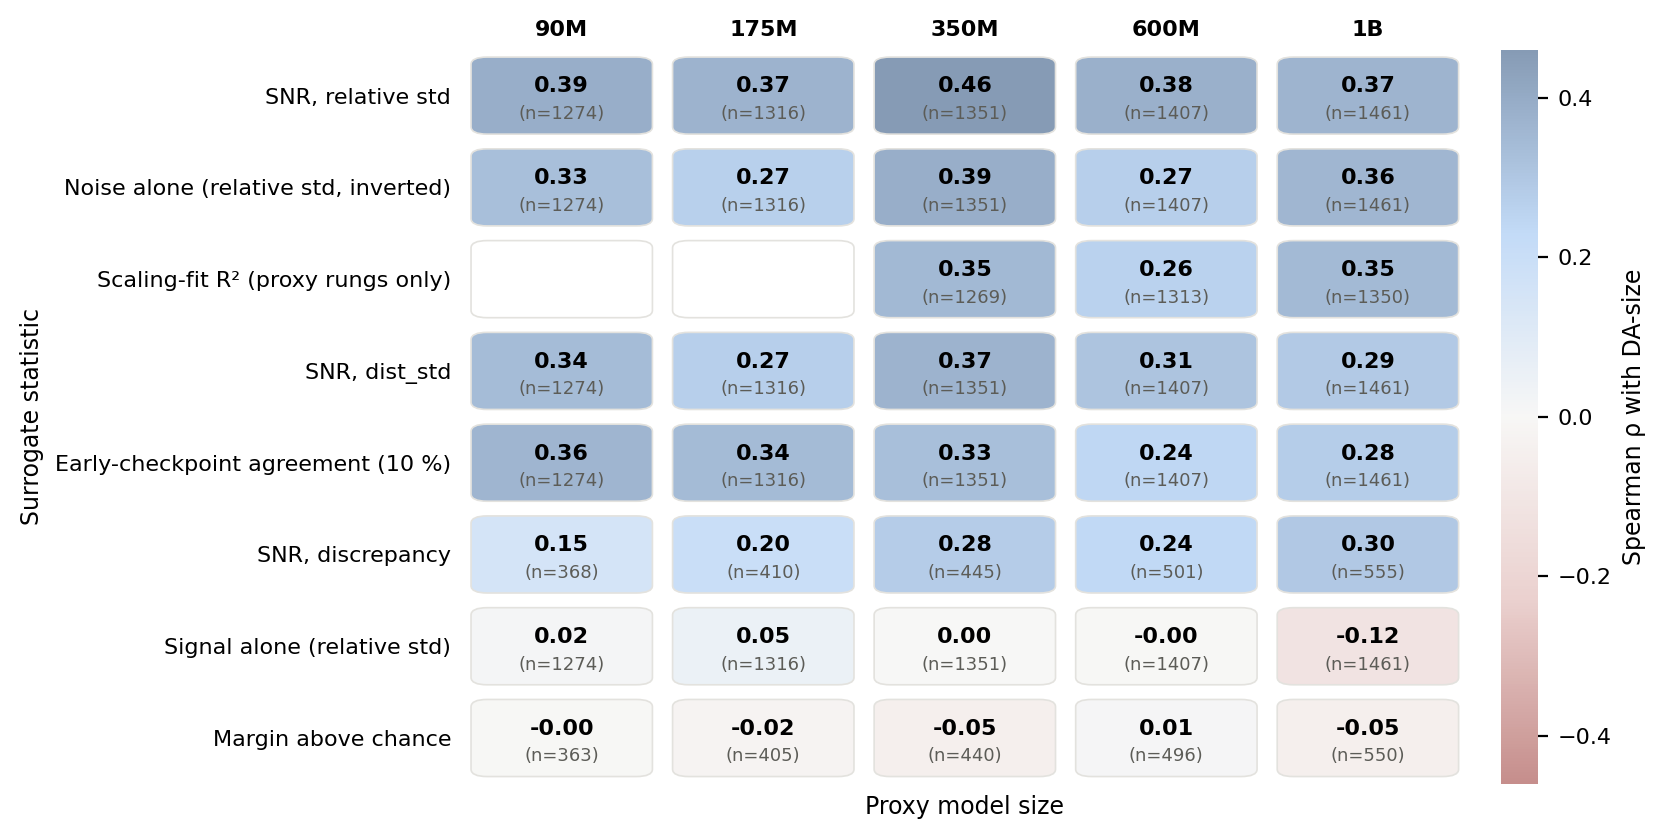
\includegraphics[width=\textwidth,height=0.8\textheight,keepaspectratio]{figures/app_rq04_surrogates_mono_axis.png}
% source: src/signal-and-noise/analysis/rq04_surrogates/pretraining/predictivity/mono_axis/rq3_surrogates_heatmap_paper.png
\caption{\textbf{On the single-axis pairs the surrogates correlate more weakly with DA-size, and the relative-standard-deviation SNR leads at every proxy size ($\rho$ 0.37--0.46).} Figure~\ref{fig:rq3} redrawn with DA-size and early-checkpoint agreement taken over the single-axis pairs of Figure~\ref{fig:rq2} instead of every pair of design variants, with the same gate (above chance at the proxy and at 1.7B) and the same bBPB twins. Early-checkpoint agreement reads 0.24--0.36 against 0.54--0.62 over every pair, and the relative-standard-deviation SNR 0.37--0.46 against 0.53--0.60. Each cell gives $\rho$ and the number of tasks $n$. The scaling-fit $R^2$ needs three model sizes, so it starts at 350M.}
\label{fig:app_rq04_surrogates_mono_axis}
\end{figure*}
